% Figure 1 float: the hero intervention. Plotting code lives in
% plotting/fig1_intervention.py; this file only wraps it for the manuscript.
\begin{figure}[tbp]
\centering
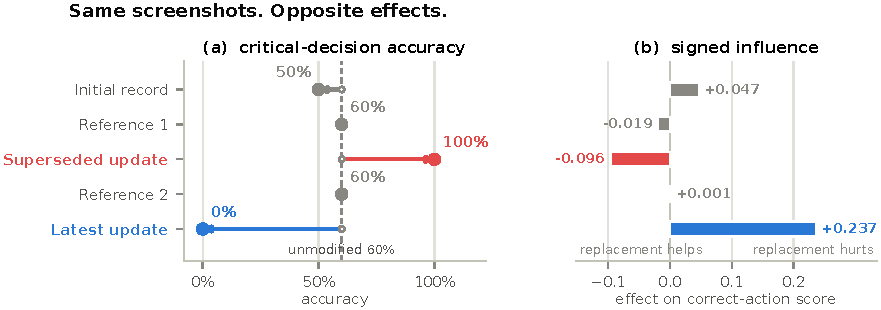
\includegraphics[width=\linewidth]{figures/fig1_intervention.pdf}
\caption{\textbf{One historical key span decides the action.} Ten paired
prefixes, frozen Qwen2.5-VL-3B-Instruct, decoder key-projection outputs at
layers 12--23. Screenshots, candidate slots, token counts and recipient
positions are identical across rows; only the source of one historical block's
key span changes. (a) Critical-decision accuracy after replacing that block with
a matched donor. (b) The same replacement's signed effect on the correct-action
score of Eq.~\eqref{eq:act}, in the units of Table~\ref{tab:pilot}. Replacing
the superseded update repairs every failure; replacing the latest update
destroys every success; the two matched references leave behaviour unchanged and
the older initial record moves it by a single prefix. Age alone therefore does
not produce the pattern.}
\label{fig:intervention}
\end{figure}
